%%---------------------------------------------------------------------------%%
%% draco-5_0_0.tex
%% Thomas M. Evans
%% $Id$
%%---------------------------------------------------------------------------%%
\documentclass[note]{ResearchNote}
\usepackage[centertags]{amsmath}
\usepackage{amssymb,amsthm,graphicx}
\usepackage[mathcal]{euscript}
\usepackage{tabularx}
\usepackage{cite}
\usepackage{c++}
\usepackage{tmadd,tmath}
\usepackage{listings}
\usepackage{color}
\usepackage{url}

%%---------------------------------------------------------------------------%%
%% DEFINE SPECIFIC ENVIRONMENTS HERE
%%---------------------------------------------------------------------------%%
%\newcommand{\elfit}{\ensuremath{\operatorname{Im}(-1/\epsilon(\vq,\omega)}}
%\msection{}-->section commands
%\tradem{}  -->add TM subscript to entry
%\ucatm{}   -->add trademark footnote about entry

\newcommand{\draco}{Draco}
\newcommand{\dracor}{\draco-6\_0\_0}
\newcolumntype{L}{>{\ttfamily}X}

\newcommand{\autoconf}{\textsf{Autoconf}}
\newcommand{\automake}{\textsf{Automake}} 
\newcommand{\CVS}{\textsf{CVS}}  
\newcommand{\make}{\textsf{Make}}
\newcommand{\gpp}{\textsf{g++}}

\newcommand{\tableText}[1]{{\raggedright #1}}


\definecolor{listingBG}{rgb}{0.95,0.95,0.95}

\lstset{language=csh,
  showstringspaces=false,
  frame=shadowbox,
  basicstyle=\footnotesize,
  rulesepcolor=\color{black},
  backgroundcolor=\color{listingBG}
}

%%---------------------------------------------------------------------------%%
%% BEGIN DOCUMENT
%%---------------------------------------------------------------------------%%
\begin{document}

%%---------------------------------------------------------------------------%%
%% OPTIONS FOR NOTE
%%---------------------------------------------------------------------------%%

\toms{Distribution}
%\toms{Joe Sixpak/XTM, MS B226}
\refno{CCS--2:10--50 (U)}
\subject{Release of \dracor}

%-------NO CHANGES
\divisionname{Computer and Computational Division}
\groupname{CCS--2:Computational Physics \& Methods}
\fromms{Kelly Thompson/CCS--2 D409\\
  Jae Chang/CCS--2 D409}
\phone{(505)665--8090}
\originator{kgt}
\typist{kgt}
\date{12/10/2010}
%-------NO CHANGES

%-------OPTIONS
%\reference{NPB Star Reimbursable Project}
%\thru{P. D. Soran, XTM, MS B226}
%\enc{list}      
%\attachments{list}
%\cy{list}
%\encas
%\attachmentas
%\attachmentsas 
%-------OPTIONS

\revisionnum{1}

%%---------------------------------------------------------------------------%%
%% DISTRIBUTION LIST
%%---------------------------------------------------------------------------%%

\distribution {

  Baker, Randal,     CCS--2  MS D409\\ 
  Budge, Kent,       CCS--2  MS D409\\
  Buksas, Michael    CCS--7  MS B287\\
  Chang, Jae,        CCS--2  MS D409\\
  Dahl, Jon,         CCS--2  MS D409\\ 
  Densmore, Jeffery, CCS--2  MS D409\\ 
  Fichtl, Erin,      CCS--2  MS D409\\
  Hungerford, Aimee, XTD--6  MS T085\\  
  Lowrie, Robert,    CCS--2  MS D413\\ 
  Rockerfeller, Gabe CCS--2  MS D409\\
  Rosa, Massimiliano, CCS--2  MS D409\\
  Thompson, Kelly,   CCS--2  MS D409\\ 
  Turner, Scott,     CCS--2  MS D409\\ 
  Urbatsch, Todd,    CCS--2  MS D409\\ 
  Warsa, James,      CCS--2  MS D409\\ 
  Wollaber, Allan,   CCS--2  MS D409\\
}

%%---------------------------------------------------------------------------%%
%% BEGIN NOTE
%%---------------------------------------------------------------------------%%

\opening

\begin{abstract}
  
  We have released \dracor.  This release marks significant changes to
  \draco.  First and foremost, ten new components have been added to
  \draco.  These components include \textsf{diagnostics},
  \textsf{fit}, \textsf{fpe\_trap}, \textsf{linear}, \textsf{min},
  \textsf{norms}, \textsf{ode}, \textsf{roots}, \textsf{shared\_lib}
  and \textsf{special\_functions}.  Two components,
  \textsf{meshReaders\_Services} and \textsf{stdheaders}, have been
  retired from \draco. The code base was updated to elminate warnings
  issued by \gpp.  Additional changes have been made to the
  \draco\ environment, organization, build system, and automatic
  documentation system, including the introduction of a proto-type
  build system based on CMake.
\end{abstract}

%%---------------------------------------------------------------------------%%

\section{\draco\ Contributors}

The following people are contributors to \draco:
\begin{center}
  \small
  \begin{tabular}{ll}
    Allan Wollaber    & \texttt{wollaber@lanl.gov} \\
    Gabe Rockerfeller & \texttt{gaber@lanl.gov} \\
    Jae Chang         & \texttt{jhchang@lanl.gov} \\
    Jeff Densmore     & \texttt{jdd@lanl.gov} \\
    Jim Warsa         & \texttt{warsa@lanl.gov} \\
    Kelly Thompson    & \texttt{kgt@lanl.gov} \\
    Kent Budge        & \texttt{kgbudge@lanl.gov} \\
    Mike Buksas       & \texttt{mwbuksas@lanl.gov} \\
    Rob Lowrie        & \texttt{lowrie@lanl.gov} \\
    Ryan McClarren    &  \\
    Seth R. Johnson   &  \\
    Tim Kelley        & \texttt{tkellyt@lanl.gov} \\
    Todd Urbatsch     & \texttt{tmonster@lanl.gov} \\
    Tom Evans         &  \\
  \end{tabular}
\end{center}

%%---------------------------------------------------------------------------%%
\newpage

\section{\draco\ Component Packages}

\dracor\ contains the following component packages:
\begin{center}
  \footnotesize
  \begin{tabular}{lp{4.0in}}
    \hline\hline
    \textsf{RTT\_Format\_Reader} & \tableText{\textsf{meshReaders}
      implementation for RTT format meshes} \\
    \textsf{c4} & \tableText{communication library for message passing interface (MPI)} \\
    \textsf{cdi} & \tableText{Common Data Interface (CDI) component} \\
    \textsf{cdi\_analytic} & \tableText{CDI analytic data component} \\
    \textsf{cdi\_gandolf} & \tableText{CDI GANDOLF wrapper for loading
    opacities from IPCRESS files} \\
    \textsf{diagnostics}  & \tableText{CPP macros for controlling runtime
      verbosity and inline timing of function calls} \\
    \textsf{ds++}         & \tableText{data structures library, DbC,
      low level functions, etc.} \\
    \textsf{fit}          & \tableText{least squares fitting routines} \\
    \textsf{fpe\_trap}    & \tableText{catch floating point signals and throw
      C++ exceptions} \\
    \textsf{lapack\_wrap} & \tableText{C++ wrapper to BLAS and LAPACK} \\
    \textsf{linear}       & \tableText{direct solvers for small linear systems} \\
    \textsf{meshReaders}  & \tableText{mesh reader interface} \\
    \textsf{mesh\_element} & \tableText{defines fundamental mesh element types
      used by meshReaders and RTT\_Format\_Reader} \\
    \textsf{min}          & \tableText{locate function minimums} \\
    \textsf{norms}        & \tableText{compute norms of vectors} \\
    \textsf{ode}          & \tableText{Runge\_Kutta, etc.} \\
    \textsf{parser}       & \tableText{generic input parser} \\
    \textsf{quadrature}   & \tableText{quadrature component} \\
    \textsf{rng}          & \tableText{random number generators and SPRNG~\cite{ce97} wrappers} \\
    \textsf{roots}        & \tableText{root finding algorithms} \\
    \textsf{shared\_lib}  & \tableText{dynamic loading of shared libraries} \\
    \textsf{special\_functions} & \tableText{math functions not provided by the
      C++ standardard library} \\
    \textsf{timestep}     & \tableText{a timestep controller component} \\
    \textsf{traits}       & \tableText{traits used by other \draco\ components} \\
    \textsf{units}        & \tableText{a physics units component} \\
    \textsf{viz}          & \tableText{interfaces to visualization tools (EnSight)} \\
    \textsf{xm}           & \tableText{glommable expression templates~\cite{fu97}} \\   
    \hline\hline 
  \end{tabular}
\end{center}

\section{Changes to individual components}
\label{sec:changes}
The following table summarizes changes to \draco\ components since
\draco-5\_0\_0. 
%% \begin{center}
%%   \begin{tabular}{lp{4.0in}}
%%     \hline\hline 
%%     stdheaders            & \tableText{retired from \draco} \\
%%     meshReaders\_Services & \tableText{retired from \draco} \\
%%     cdi\_eospac           & \tableText{not included as part of
%%       \dracor\ because of EOSPAC/FORTRAN compiler issues; will be
%%       re-integrated when EOSPAC 6.0 is released} \\
%%     ds++                  & \tableText{added reference counted field
%%       class (\texttt{RCF}) and a light-weight vector
%%       (\texttt{Vector\_Lite})} \\  
%%     Draco Build System & \tableText{autodoc generation enhanced; MPI
%%       defaults on LINUX removed; added middleware vendor option for
%%       clients of the build system; see \S~\ref{sec:dbs} for details} \\
%%     tools & \tableText{added several new tools including
%%       \texttt{check\_for\_tags.py}, \texttt{numdiff.py},
%%       \texttt{update\_release\_tags.py}, and \texttt{profiler.py};
%%       updated \texttt{launchtest} script to work for IBM and use a
%%       cleaner implementation} \\
%%     \hline\hline 
%%   \end{tabular}
%% \end{center}

\subsection{c4}
\label{changes:c4}
\begin{itemize}
\item Added \texttt{global\_containers.hh} which provides functions
  for global manipulation of sets and maps.
\item A new class \textsf{Processor\_Group} has been added. This class
  is useful for managing different kinds of decompositions in a single
  program. 
\item A new class \textsf{Termination\_Detector} has been added. This
  class is a general-purpose terminator for indeterministic parallel
  algorithms. 
\item Encapsulate platform specific header files to better support
  non-Linux systems.
\item Added some scatter and gather operations with multiple
  convenience interfaces.
\item Added routines to manage swapping of data between processors.
\item Update routines to correctly treat the case where message size
  is zero.  Prevent safe \texttt{\&v[0]} type operations so that
  instrumentation of the code doesn't trip over itself.
\item Replace the use of \texttt{rtt\_c4::finalize()} with
  \texttt{rtt\_c4::abort()} when it appears in a catch block in the
  unit tests. 
\item Added a variable to serve as the source/destination of a null
  process.
\item Added function \texttt{Compare} for equivalence testing of
  values on different processors.
\item Added base class in \texttt{Send\_Receive} to support custom
  data communicators.
\item Added utilities to support creating data mapping operators.
\item Removed \texttt{wait()} from \texttt{C4\_Req} destructor; this
  was creating non-exception safe code in parallel execution modes.
\item Added \textsf{MPI\_Probe} implementation as a generic
  \texttt{blocked\_probe} function.
\item Remove deprecated \texttt{C4::send()} and \texttt{C4::recv()}
  from the old C4 namespace.
\item \texttt{abort()} function added in \draco-5\_6\_0.
\end{itemize}

\subsection{cdi}
\label{changes:cdi}
\begin{itemize}
\item Provide support for Opacity Distribution Functions
  (ODF)~\cite{ccs2:08-52}. This capability supports the idea of
  multiple opacity {\it bands} per group.  
\item Provide functions that return Planckian and Rosseland integrals
  for all groups in a group structure.
\item Added a new full-spectrum integrator which just integrate the
  Planckian over all groups in the group structure.
\end{itemize}

\subsection{cdi\_analytic}
\label{changes:cdi-analytic}
\begin{itemize}
\item Provide support for Opacity Distribution Functions
  (ODF)~\cite{ccs2:08-52}.  
\item Provide support for frequency dependant polynomial models.
\end{itemize}

\subsection{cdi\_gandolf}
\label{changes:cdi-gandolf}
\begin{itemize}
\item Provide support for Opacity Distribution Functions
  (ODF)~\cite{ccs2:08-52,gandolf}.
\end{itemize}

\subsection{ds++}
\label{chagnes:dsxx}
\begin{itemize}
\item Add class \textsf{Field\_Traits}. This class is useful in some
  template code dealing with real fields.  The \texttt{to\_string}
  function is a convenient converter from numeric types to
  \texttt{std::string}.
\item Add class \textsf{Homogeneous\_New}.
\item Provide some low level functions for portability and easier
  templatization.  See \texttt{ags.hh}, \texttt{cube.hh},
  \texttt{dim.hh}, \texttt{isFininte.hh}, \texttt{pythag.hh},
  \texttt{value.hh}, \texttt{sign.hh}, \texttt{square.hh},
  \texttt{to\_string.hh} \texttt{conj.hh} and \texttt{dbc.hh}.
\item Provide support for hiding/exposing symbols in shared object
  libraries (\texttt{DLL\_SHARED} macro).  See
  \texttt{ds++/config.h.in} for details.
\item The Design-by-Contract macro \texttt{REMEMBER} is now defined
  anytime \texttt{DBC != 0} .
\item Provide a new header, \texttt{path.hh}, that encapsulates path
  separation symbols along with a few other file system related
  behaviors.
\item Provide a new class \textsf{Slice} that allows viewing a slice
  of an arbitrary container.
\item Added a collection of ocmpiler specific macros.
\item Provide endian conversion functions and support in serializatoin
  operators.
\item Provide overflow protected division.
\item Provide function for searching for data in vectors.
\item Provide \textsf{Index\_Converter} which maps multiple dimension
  indices to and from a single dimensional version.
\item New classes \textsf{DBC\_Ptr}, \textsf{Safe\_Divide},
  \textsf{Safe\_Ptr}, \textsf{Thin\_Ptr} added in \draco-5\_7\_0.
\end{itemize}

\subsection{fpe\_trap}
\label{change:fpe-trap}
\begin{itemize}
\item The functionality of this package was inadvertantly disabled on
  Linux64 due to an autoconf script defect.  The package has been
  reactivated.
\item On Darwin, it appears that the SIGFPE is caught, but the
  operating system still aborts the process and pops up a GUI
  information box to this effect.  There is no clear path forward to
  fix this problem.
\item New package in \draco-5\_9\_0.
\item Remove dependency on \textsf{c4}.
\end{itemize}

\subsection{mesh\_element}
\label{changes:mes-element}
\begin{itemize}
\item Added generic element identifier and support.
\end{itemize}

\subsection{meshReaders}
\label{changes:meshReaders}
\begin{itemize}
\item Provide support for general Polygon type mesh element.
\end{itemize}

\subsection{meshReaders\_Services}
\label{changes:meshReaders-Services}
The stdheaders component has been retired from \draco.

\subsection{stdheaders}
\label{changes:stdheaders}
The stdheaders component has been retired from \draco\ because all
currently supported compiler provide sufficient support of the STL
library.  Early versions of \draco\ were built with compilers that did
not provide STL functions in the \texttt{std::} namespace and this
package addressed those deficiencies.

\subsection{parser}
\label{changes:parser}
\begin{itemize}
\item Add \textsf{Abstract\_Class\_Parser}, \textsf{Class\_Parser}
  \textsf{Constant\_Expression} and \textsf{Expression} classes.
\item New package for \draco-5\_8\_0.
\item Added ability to parse \texttt{rtt\_mesh\_element::Geometry}
  specification. 
\item Added exception handling.
\item Better parallel/serial integration.
\item Integration with the \textsf{units} package.
\end{itemize}

\subsection{quadrature}
\label{changes:quadrature}
\begin{itemize}
\item Refactored the \textsf{Transport\_Model} and
  \textsf{Radiation\_Package} interface.
\item All quadrature sets are now normalized so that their weights sum
  to unity.
\item Provided the triangular Chebyshev-Legendre quadrature set.
\item Provided the 1D level-symmetric set in the
  \textsf{SquareChebyshevLegendre}. 
\item Extended \texttt{Discrete\_To\_Moment} and 
  \texttt{Moment\_To\_Discrete} to support 3D.
\item Replace the use of {\it angle} with {\it ordinate} everywhere
  but \texttt{Angle\_Operator}.
\item Add checks to prevent the use of 1-D quadrature for axisymmetric
  geometry. 
\item Added the ability to generate quadratures from a
  \textsf{Token\_Stream}. 
\item Provide ability to reflect 2D square quadratures.
\item Provide \texttt{quadCreate} function that accepts a
  \textsf{Token\_Stream} as an argument.  
\item Provide two different methods for generating the
  discrete-to-moment matrix (tradiational Sn and Morel's Galerkin
  method).  Also provided three new mechanisms for generating
  moment-to-discrete matrix (tranditional Sn, Morel's Galerkin and an
  experimental SVD method).
\item Added 1D-to-2D quadrature permutations.
\item Added 1D Double Gauss quadrature.
\item Added 1D Lobatto quadrature.
\end{itemize}

\subsection{rng}
\label{changes:rng}
\begin{itemize}
\item Added some convenient pseudo-random number generators:
  \textsf{Halton\_Sequence}, \textsf{Halton\_Subrandom\_Generator},
  \textsf{Sobol\_Sequency} and \textsf{LC\_Subrandom\_Generator}.
\item Extracted, rewrote and implemented parts of the SPRNG library to
  provide a more efficient inline random number stream.
\item Extended unit tests to provide better function point coverage.
\item Commented out unused functions and function arguments as
  identified by g++.
\end{itemize}

\subsection{RTT\_Format\_Reader}
\label{changes:RTT-Format-Reader}
\begin{itemize}
\item Added support for general Polygon type mesh element.
\item Fixed a bug in the logic of the \texttt{redefineCells}
  function. 
\item Added triangle and quadratic line elements.
\end{itemize}

\subsection{special\_functions}
\label{changes:special-functions}
\begin{itemize}
\item Eliminate code that will always overflow (factorial).
\item Change the signature of KroneckerDelta so that it returns an
  unsigned integer.
\item Provide static integer power function.
\item Provide spherical harmonics functions.
\item Provide KronekerDelta and factorial functions.
\item Provide x-to-the-power functions.
\item Added more Fermi-Dirac functions, including: F1, F12, F12inv,
  F2, F2inv, F3, F32, F4, FM12, F\_eta, and F\_eta\_inv.
\end{itemize}

\subsection{units}
\label{changes:units}
\begin{itemize}
\item Added {\it cgsh} and {\it cgmu} unit systems.
\item Added output unit system specification.
\end{itemize}

\subsection{viz}
\label{changes:units}
\begin{itemize}
\item Added unit tests to bring the function point code coverage above
  80\%.
\item Update code base to make correct use of signed vs. unsigned
  integer types.
\item Wrap OS specific command (e.g.: \texttt{mkdir} or \texttt{rm})
  as CPP macros defined in \texttt{config.h}.
\end{itemize}
%------------------------------------------------------------------------------%

\section{Defects}
Here is a list of known defects:
\begin{itemize}
\item The \texttt{autodoc} target is currently broken for the
  autoconf-based build.
\end{itemize}

\noindent Here is a list of known bug fixes:
\begin{itemize}
\item Fixed memory leak in \textsf{DBC\_Ptr} classes
  (\textsf{Safe\_Ptr}) and updated testing.  Fixed an assignment error
  in \textsf{Thin\_Ptr}.
\item Fixed a bug in the anisotropic moment-to-discrete computation
  for starting directions (\url{quadrature/QuadServices.cc}).
\end{itemize}

%------------------------------------------------------------------------------%

\section{Design}

There are no inter/intra-component cyclic dependencies in \draco.  The
levelized graph for \dracor\ components is shown in
Fig.~\ref{fig:level}.  The diagram includes the 10 new packages.  It
should be noted that changes to the \textsf{rng} component require it
to link against the \textsf{GSL}\footnote{GNU Scientific Library}.
This is a new dependency.
\begin{figure}
  \label{fig:level}
  \centerline{
    \includegraphics[height=5.5in]{level-6_0_0.ps}}
  \caption{\dracor\ levelized component graph.  Dotted lines signify
    that the dependency if only required for testing.}
\end{figure}

%------------------------------------------------------------------------------%

\section{Code Statistics}


%% tools/count_loc.sh

%% Counting lines of source code --
%% Directory:  /var/tmp/kgt/draco600/draco600
%% Date     :  Thu Dec 9 17:55:14 MST 2010

%%                  Total C++ source: 39210
%%    C++ source in test directories: 22161
%%       C++ contract specifications: 1443
%%                      C++ comments: 43076
%%              Total Fortran source: 0
%%                  Fortran comments: 0
%%               LaTeX Documentation: 14758
%%                       HTML source: 0
%%                         Text docs: 5811
%%        Build system script source: 12126
%%    Executable shell script source: 3352
%%            Executable Perl source: 1867
%%                     Python source: 4172
%%                     Expect source: 0
%%                      Elisp source: 6583


Lines-of-Code (LOC) statistics for all \draco\ releases are are shown
in Fig.~\ref{fig:stats}.  The large drop between \draco-4\_0\_0 and
\draco-5\_0\_0 is due to the removal of the \textsf{mc} and
\textsf{imc} packages. The aggregate LOC statistics for \dracor\ are:
\begin{center}
  \begin{tabular}{|l|l|} \hline
    Total component package source code & 39210 \\
    Total unit test code & 22161 \\
    Total DBC statements & 1443 \\
    Total comments & 43076 \\
    \hline
  \end{tabular}
\end{center}
\begin{figure}
  \label{fig:stats}
  \centerline{
    \includegraphics[width=6in]{draco600-loc-history.ps}}
  \caption{LOC statistics for \dracor\ component packages.}
\end{figure}
Table~\ref{tab:loc} shows LOC metrics for each \draco\ component in
\dracor.  LOC metrics are stored in \draco\ in
\texttt{draco/doc/code\_stats}.
\begin{table}
  \caption{
    LOC metrics for component packages in \dracor.  DBC LOC refers to
    Design-by-Contract$^{\copyright}$ statements. 
  }
  \label{tab:loc}
  \begin{center}
    \begin{tabular}{llll}\hline\hline
      \multicolumn{1}{c}{Component} &
      \multicolumn{1}{c}{Source LOC} &
      \multicolumn{1}{c}{DBC LOC} &
      \multicolumn{1}{c}{Test LOC} \\\hline
      RTT\_Format\_Reader &     2408     &       19      &      1063     \\
      c4                 &      2702     &       86      &      1294     \\
      cdi                &      1566     &       82      &      1122     \\
      cdi\_analytic      &      1436     &      110      &       771     \\
      cdi\_gandolf       &      2150     &       45      &      1248     \\
      diagnostics        &       333     &        4      &       267     \\
      ds++               &     11155     &      337      &      8147     \\
      fit                &        95     &        3      &        56     \\
      fpe\_trap          &       117     &        5      &        51     \\
      lapack\_wrap       &       193     &       37      &       116     \\
      linear             &      1083     &       51      &       462     \\
      meshReaders        &       454     &       16      &       261     \\
      mesh\_element      &      1270     &       36      &       727     \\
      min                &       631     &        2      &       399     \\
      norms              &       282     &        4      &       160     \\
      ode                &       193     &        6      &        86     \\
      parser             &      3182     &      218      &      1475     \\
      plot2D             &       329     &       30      &        76     \\
      quadrature         &      3106     &      192      &      1195     \\
      rng                &       355     &       18      &       184     \\
      roots              &       670     &        8      &       219     \\
      shared\_lib        &       184     &       12      &       118     \\
      special\_functions &       976     &       10      &       490     \\
      timestep           &       533     &       16      &       196     \\
      traits             &       134     &       9       &       47      \\
      units              &      1401     &       11      &       1186    \\
      viz                &       680     &       47      &       209     \\
      xm                 &       414     &       4       &       257     \\
      \hline\hline
    \end{tabular}
  \end{center}
\end{table}

%% cd draco/src
%% for dir in `/bin/ls -1 -d */`; do echo "---- $dir ----''; (cd $dir;\
%% ../../tools/count_loc.sh); done 




With the adoption of the \textsf{Bullseye} coverage analysis tool, we
are better able to track unit-test coverage of \draco\ components.
The goal is to achieve 100\% functional test coverage for each \draco\
component.  Table~\ref{tab:coverage} gives functional and conditional
point coverage for \dracor.
%%---------------------------------------------------------------------------%%
%% coverage table for draco-6_0_0
%%---------------------------------------------------------------------------%%


\begin{table}
  \caption{
    Unit-test coverage in \dracor.  C/D Coverage refers to conditional
    statements.  We strive for 100\% function point coverage.  
  }
  \label{tab:coverage}
  \begin{center}
    \begin{tabular}{lllll}\hline\hline
      \multicolumn{1}{c}{Component} &
      \multicolumn{1}{c}{Function Coverage} &
      \multicolumn{1}{c}{Percent (\%)} &
      \multicolumn{1}{c}{C/D Coverage} &
      \multicolumn{1}{c}{Percent (\%)} \\\hline

RTT\_Format\_Reader &   316 /   322 &  98 &    273 /   356 &  76 \\
c4                  &   169 /   173 &  97 &    279 /   336 &  83 \\
cdi                 &    40 /    40 & 100 &     27 /    30 &  90 \\
cdi\_analytic       &   105 /   106 &  99 &    105 /   110 &  95 \\
cdi\_gandolf        &   130 /   131 &  99 &    154 /   232 &  66 \\
diagnostics         &    22 /     26 &  84 &     81 /   168 &  48 \\
ds++                &   671 /    713 &  94 &    608 /   716 &  84 \\
fit                 &     2 /     2  & 100 &     15 /    16 &  93 \\
fpe\_trap  &              3 /     3  & 100 &      4 /    11 &  36 \\
lapack\_wrap   &         11 /    17  &  64 &      0 /     0 & \\
linear  &                16 /    17  &  94 &    320 /   392 &  81 \\
meshReaders  &           16 /    16  & 100 &    127 /   172 &  73 \\
mesh\_element  &         25 /    25  & 100 &    157 /   205 &  76 \\
min  &                   10 /    10  & 100 &    137 /   154 &  88 \\
norms  &                 26 /    27  &  96 &     21 /    34 &  61 \\
ode  &                    6 /     6  & 100 &     29 /    32 &  90 \\
parser  &               226 /   264  &  85 &    965 /  1345 &  71 \\
plot2D  &                22 /    30  &  73 &     46 /    76 &  60 \\
quadrature  &           162 /   170  &  95 &    421 /   508 &  82 \\
rng  &                   59 /    68  &  86 &     63 /    70 &  90 \\
roots  &                  9 /     9  & 100 &    252 /   312 &  80 \\
shared\_lib  &           11 /    13  &  84 &      7 /    10 &  70 \\
special\_functions  &    28 /    28  & 100 &    161 /   162 &  99 \\
timestep  &              49 /    62  &  79 &     88 /   178 &  49 \\
traits  &                17 /    17  & 100 &      0 /     0 & \\
units  &                 83 /    83  & 100 &     58 /    58 & 100 \\
viz  &                   23 /    26  &  88 &    129 /   168 &  76 \\
xm  &                    56 /    58  &  96 &     29 /    32 &  90 \\
      \hline
      {\bf Total} & {\bf 2313/2462} & {\bf 93} & {\bf 4556/5883} & {\bf 77} \\

      \hline\hline
    \end{tabular}
  \end{center}
\end{table}

%%---------------------------------------------------------------------------%%
%% end of coverage table
%%---------------------------------------------------------------------------%%


%%---------------------------------------------------------------------------%%

\section{\draco\ Build System}
\label{sec:dbs}

The traditional autoconf-based \draco\ Build System (DBS) has
undergone some significant changes.  The most significant changes are
support for new platforms and compiler sets, new vendor libraries and
more automation.  The build system required the developer to provide
fewer command line arguments and will choose reasonable defaults in
most cases.  Ultimately, the developer still has the ability to avoid
using any default value by specifying his or her own options on the
configure line.  Specific changes to the build system are itemized
here: 
\begin{itemize}
\item Separated the build and testing phases in the
  \texttt{Makefiles}.  This change is needed becuase of limitations on
  ASC hardware where we build on the front end but run the tests on
  the worker nodes.  \texttt{make} alone will build the libraries.
  \texttt{make all} will build all libraries and unit tests, but not
  run them.   \texttt{make check} will compile all libraries and unit
  tests and run all unit tests.  \texttt{make run} will run the tests
  without trying to build anything.
\item Provided support for building a stubbed out version of
  \textsf{cdi\_gandolf}.
\item Changed the build system so that it tries to determine if either
  \texttt{-lgfortran} or \texttt{-lg2c} are needed on the link lines.
\item No longer store generated \texttt{aclocal.m4} files in \CVS.
\item Support for STLPort cleaned up in \draco-5\_5\_0.
\item Simplified autoconf-based build system to eliminate the
  requirement for lengthy configure commands.  Most options are now
  defaulted to reasonable values.
\item Added support for Intel compilers (icc, icpc, ifort).
\item Added support for RoadRunner's PPE cross compiler, ppu-g++.
\item Added support for gcc-4+ including gfortran.
\item Improved support for IBM xlc compiler and AIX.
\item Improved support for PGI compilers (pgcc, pgCC, pgfort)
\item Added support for linking FORTRAN main programs.
\item Added support for new vendors including Silo, ParMetis, NDI and
  SuperLU\_DIST.
\item Added unofficial support for Darwin (PPC and Intel) and MSVC on
  Windows (note that not all packages can be compiled on these
  architectures).
\item Many \texttt{config.h.in} files were modified to support
  configuration with either \textsf{autoconf} or \textsf{CMake}. A new
  define for \texttt{AUTOCONF} is found in both \texttt{configure.ac}
  files and in \texttt{config.h.in} to keep the 2 build systems
  working simultaneously.
\item Corrected a glitch in the config scripts that assumed that
  \texttt{CXX} would be the name of a comiler without the full path
  prepended.  On the HPC hardware or when using \draco\ modules, this
  variable always uses the full path to the compiler.
\end{itemize}

Additionally, a prototype \textsf{Scons} build system was implemented
while porting Jayenne codes to RoadRunner.  While this build system
remains mostly intact, it is not being adopted or maintained for this
release. A prototype \textsf{CMake} build system has been added
recently and will be evaluated early in 2011 to determine if
\draco\ development will move to the CMake-based system.  The
CMake-based system required less scripting code to be supported by the
\draco\ team, it has better dependency checking, better parallel build
support, a mature testing system and suppport for dashboard reporting.
The current prototype reports results to \url{coder.lanl.gov/cdash}.

Two new top-level configure options have been added to the build
system.  The first turns up the warning level for \gpp\ and the second
provide additional checks (similar to STLPort) at run time.  The new
options are detailed below:
%
\begin{center}
  \footnotesize
  \begin{tabular}{lp{4.0in}}
    \hline\hline
\texttt{--enable-all-warnings} & 
     \tableText{For g++, this option turns on -Wall and -Wextra.
       \draco\ was updated to build cleanly with theses flags, but
       they are not the default yet.} \\ 
\texttt{--enalbe-glibcxx-debug} &
     \tableText{For g++, this option uses the debug GLIBCXX
       libraries.  This option provides bounds checking for STL
       containers and more.  It addes the following defines to
       \texttt{CXXFLAGS}: \texttt{-D\_GLIBCXX\_DEBUG
         -D\_GLIBCXX\_DEBUG\_PEDANTIC}. } \\
    \hline\hline
  \end{tabular}
\end{center}

It is no longer required to use configure options like
\texttt{--with-mpi-inc --with-mpi-lib}.  The build system will set
these values automatically if your environment is set correctly. (It
will be if you use the environment/Modules!)  That is, you will need
to set \texttt{MPI\_INC\_DIR} and \texttt{MPI\_LIB\_DIR} in your
environment before running configure.  If MPI is not found in your
environment, the build system will automatically default to the
\texttt{--with-c4=scalar} option.  This trend will hold true for other
vendor libraries as well (GSL, Trilinos, LAPACK, etc.).  If a vendor
library is not found, then dependent \draco\ components will be
omitted.  For example, if GSL is not found by the build system then
\textsf{quadrature}, \textsf{rng} and \textsf{special\_functions} will
not be built.

%%---------------------------------------------------------------------------%%

\section{\draco\ Directory Structure}

The current \draco\ directory structure is shown below:
\begin{lstlisting}[basicstyle=\footnotesize, xleftmargin=2.0in, 
  xrightmargin=2.0in]
draco/
    src/
        ds++/
        c4/
        ...
    doc/
        gettingStarted/
        releases/
        ...
    tools/
    autodoc/
    config/
    environment/
        Modules/
        bashrc/
        bibfiles/
        bibtex/
        bin/
        elisp/
        latex/
        python/
        share/
        templates/
\end{lstlisting}
Table~\ref{tab:envdir} describes the purpose of each of the
\texttt{environment} directories in detail.  The rest of the
\draco\ directory structure is self-explanitory.
\begin{table}[!ht]
  \caption{
    Descriptions of the directories in \texttt{draco/environment}.
    The \draco\ development environment is entirely encapsulated
    within the \texttt{environment} directory.
  }
  \label{tab:envdir}
  \begin{center}
    \begin{tabular}{lp{3in}}\hline\hline
      \multicolumn{1}{c}{Directory} & 
      \multicolumn{1}{c}{Description} \\ \hline
      
      \texttt{Modules} & \tableText{initialization scripts for the
        module command and module scripts that know how to load and
        unload various modules for vendors, compilers, tools, etc.} \\
      
      \texttt{bashrc} & \tableText{A set of default bash setup scripts
        taht can be sourced by \draco\ developers to quickly setup
        their environment.} \\

      \texttt{bibfiles} & \tableText{bibliography databases
        (\texttt{.bib} files)} \\ 
      
      \texttt{bibtex} & \tableText{bibliography style files
        (\texttt{.bst} files)} \\
      
      \texttt{elisp} & \tableText{the \draco\ GNU Emacs/XEmacs macro
        definitions.} \\
      
      \texttt{latex} & \tableText{latex class and style files
        (\texttt{.cls} and \texttt{.sty} files)} \\ 

      \texttt{templates} & \tableText{code, build system, and
        documentation templates.} \\

      \hline\hline
    \end{tabular}
  \end{center}
\end{table}

The \draco\ Build System (DBS), encapsulated within
\texttt{draco/config}, is separate from the \draco\ development
environment sitting in \texttt{environment}.  This separation exists
because \texttt{config} is required to build the code whereas
\texttt{environment} is only required to develop the code.  Thus,
clients who only wish to link \draco\ components do not require
\texttt{environment}; they do need \texttt{config}.

\newpage
Recommended incorporation of the bashrc environment (assuming draco is
checked out at \texttt{~/draco}).
\begin{lstlisting}[basicstyle=\footnotesize, xleftmargin=0.5in, 
  xrightmargin=0.5in]
#!/bin/bash
# file: ~/.bashrc

# basic setup including sourcing of /etc/bashrc goes first.

# if interactive:
if test -f ~/draco/environment/bashrc/.bashrc; then
   source ~/draco/environment/bashrc/.bashrc
fi

# More setup goes here (possibly altering what is in the default
# scripts). 
\end{lstlisting}

Recommended incorporation of the elisp environment:
\begin{lstlisting}[basicstyle=\footnotesize, xleftmargin=0.5in, 
  xrightmargin=0.5in]
%.emacs

% custom settings go here

;; Load the Draco modes.
(setq draco-env-dirs (list
		      "~/.emacs.d/draco/"
		      "~/.emacs/"))
(load-library "~/.emacs.d/draco/draco-setup")

% more customization goes here
\end{lstlisting}

\newpage
Sample use of the \texttt{module} commands:
\begin{lstlisting}[basicstyle=\footnotesize, xleftmargin=0.5in, 
  xrightmargin=0.5in]
% module clear 

% module avail
--------------- ~/draco/environment/Modules/modulefiles ----------------
cmake/2.8.1   doxygen/1.6.3 module-cvs    null          use.own
cmake/2.8.2   doxygen/1.7.1 module-info   numdiff/5.2.1
cmake/2.8.3   graphviz      modules       p7zip/9.04

--------------- ~/draco/environment/Modules/ccs-Linux64 ----------------
BLACS                    gcc/4.3.0                openmpi/1.3.3
ParMetis/3.1             gcc/4.3.4                pcg/1.0
ParMetis/3.1.1           gcc/4.4.4                pgi/10.4
SCALAPACK                gcc/4.5.0                pgi/7.0-5
SuperLU_DIST/2.3         grace                    pgi/9.0-3
SuperLU_DIST/2.4         gsl                      python/2.5.1
boost/1.43.0             hypre/1.8.2b             totalview/8.4.1-7
bullseyecoverage/7.13.44 hypre/2.0.0              totalview/8.8.0-2
dia/0.97                 intel/10.0.023           trilinos/10.4.0
dot                      lapack/atlas-3.8.3       trilinos/9.0.2
emacs/23.2               mpich/1.2.4              valgrind/3.5.0
gandolf                  mpich/1.2.5
gcc/4.1.1                ndi

% module load modules cmake doxygen graphviz numdiff p7zip dia dot \
          emacs gandolf gcc grace gsl openmpi python totalview \
          valgrind
% module list
Currently Loaded Modulefiles:
  1) modules             7) dia/0.97           13) gsl
  2) cmake/2.8.3         8) dot                14) openmpi/1.3.3
  3) doxygen/1.7.1       9) emacs/23.2         15) python/2.5.1
  4) graphviz           10) gandolf            16) totalview/8.8.0-2
  5) numdiff/5.2.1      11) gcc/4.5.0          17) valgrind/3.5.0
  6) p7zip/9.04         12) grace

% module switch gcc gcc/4.4.4

% module unload grace

# Vendor modules setup environment that helps the build system:
% echo $MPI_INC_DIR
MPI_INC_DIR=/ccs/codes/mpi/openmpi/Linux64/1.3.3/include

% echo $MPI_LIB_DIR
MPI_LIB_DIR=/ccs/codes/mpi/openmpi/Linux64/1.3.3/lib
\end{lstlisting}


%%---------------------------------------------------------------------------%%
\section{Draco Development Environment}
The \draco\ development environment has been updated with this
release.  This update inclues the introduction of \textsf{modules} to
assist in switching between compilers and setting up developer's
environment to use supported vendors (MPI, Trilinos, etc.).  

\subsection{Elisp}

The elisp module was updated to provide better support for GNU Emacs 22.4.

\subsection{Bash}

The bash scripts have been updated to automatically load the modules
environment.  Updates for new CCS and HPC systems are also included.

\subsection{\LaTeX}

There are no significant changes to the provided \LaTeX\ environment.

\subsection{Modules}

The modules\footnote{See http://modules.sourceforge.net} environment
is new for this release.  The recommended use is to source the
modules/init files from your startup scripts.  Once incorporated into
your shell environment you can use \texttt{module avail} to list
available modules.  \texttt{module load} is used to activate a
particular module's settings.

%%---------------------------------------------------------------------------%%

\section{Quick Start Instructions}

Prerequisits: You must be in the \textsf{radtran} and \textsf{draco} Unix file
sharing groups.

\begin{verbatim}
% export CVSROOT=/ccs/codes/radtran/cvsroot
% cvs co -P draco
% ./draco_config
% cd $build_dir
% ~/draco/configure --prefix=<dir>
% make check
\end{verbatim}

%%---------------------------------------------------------------------------%%

\nocite{rn98046}
\nocite{xtm:9936}
\nocite{draco-3_0_0}
\nocite{draco-4_0_0}
\nocite{draco-5_0_0}
\bibliographystyle{rnote}
\bibliography{../../environment/bibfiles/draco}
 
\closing
\end{document}

%%---------------------------------------------------------------------------%%
%% end of draco-5_0_0.tex
%%---------------------------------------------------------------------------%%
